%==============================================================================
%  PART 1 --- FOUNDATIONS
%  Chapters: Introduction | Background & Related Work | Data Model & Dataset
%==============================================================================

\chapter{Introduction}
\label{ch:intro}

\section{Context and motivation}
Prediction markets are exchanges on which participants trade contracts whose
payoff is tied to the outcome of a future, verifiable event. Because a rational
trader buys a ``\textsc{Yes}'' share whenever its price is below their subjective
probability of the event and sells when it is above, the equilibrium price of a
binary contract behaves as a continuously updated, money-weighted estimate of the
event's probability~\cite{wolfers2004prediction,berg2008prediction}. Among
contemporary platforms, \emph{Polymarket} has become one of the most liquid and
widely watched venues, hosting contracts on politics, macroeconomics, crypto-asset
price levels, sports, and current affairs. The resolved history of these contracts
provides something rare in forecasting research: a large set of events with a
\emph{known ground-truth outcome} and a \emph{full price trajectory} leading up to
it.

In parallel, a large share of the public reasoning \emph{about} these same events
happens on social-media platforms --- Reddit threads, Telegram channels, and posts
on X (formerly Twitter). This discourse encodes sentiment, narratives, rumours, and
occasionally genuine private information. A long line of work has asked whether such
signals anticipate real-world or market outcomes, with results ranging from
optimistic~\cite{bollen2011twitter,salathe2012assessing} to sharply
qualified~\cite{tetlock2007giving}. The question is far from settled, and it is
exactly the question this project investigates in the specific, well-instrumented
setting of Polymarket.

\section{Research question and objectives}
The project is organised around a single, deliberately conservative research
question:

\keyfinding{\textbf{Do social-media signals provide \emph{incremental} predictive
value over market-implied probabilities, and if so, in which thematic domains, on
which platforms, and over which time windows?}}

\noindent The emphasis on \emph{incremental} value is the methodological core of the
work. It is easy --- and uninteresting --- to show that social sentiment correlates
with an outcome when the market price already encodes that information. The
scientifically meaningful test is whether social features improve a forecast
\emph{on top of} the market price, under an evaluation that forbids any leakage of
post-resolution information. We therefore frame PolySignal not as an attempt to
``beat Polymarket'', but as an analytical layer that quantifies social context and
submits it to a controlled, falsifiable test.

\noindent Operationally, the work pursues the three goals set out by the assignment:
\begin{enumerate}
  \item \textbf{Dataset construction (Task 1).} Build a reproducible ingestion
  pipeline that collects resolved Polymarket contracts and their price time series,
  collects longitudinal social discourse, links posts to contracts, normalises and
  enriches the text, and stores everything in a queryable format.
  \item \textbf{Analytical study (Task 2).} Characterise the contracts and the
  discourse descriptively; study the temporal relationship between social signals
  and price movements; compare platforms and domains; and expose the results through
  an interactive dashboard.
  \item \textbf{Outcome prediction (Task 3, optional).} Engineer social features and
  evaluate, with temporal cross-validation and explicit ablations, whether they add
  predictive value over the market price.
\end{enumerate}

\section{Design philosophy}
Four principles shaped every component and are worth stating up front, because they
explain many concrete choices later in the report.

\begin{description}[leftmargin=1.4em,style=nextline]
  \item[Deterministic core, optional intelligence.] The full pipeline runs
  end-to-end \emph{without} any call to an external language model. LLM-assisted
  steps exist only as opt-in, cached verifiers layered on top of a deterministic
  baseline. This guarantees reproducibility and decouples our results from a paid,
  non-deterministic dependency.
  \item[Time discipline and no leakage.] Every record carries a timezone-aware
  timestamp, and every forecasting or backtesting step enforces a strict
  ``no information from the future'' rule: a market's resolution can never reach a
  feature, and a post published after a contract closed can never count as evidence
  for it.
  \item[No invented data.] The system never fabricates posts, markets, or labels to
  inflate coverage. Empty or sparse cells are reported honestly --- a property that
  proves essential when we discuss the coverage limitations in
  \Cref{ch:limitations}.
  \item[Honest reporting.] We report a negative predictive result in full, with its
  diagnostics, rather than selecting a favourable slice. A robust null result, in a
  field prone to over-optimistic claims, is itself a contribution.
\end{description}

\section{Scope decisions}
\label{sec:scope}
Two scope decisions are load-bearing and are justified in detail where they arise;
we summarise them here so the reader can keep them in mind.

\paragraph{Platforms: all three collected, Telegram-dominated.}
The assignment names three platforms, and the pipeline implements a collector for
each: \textbf{Telegram} (via the official MTProto API, using Telethon),
\textbf{Reddit} (via compliant public-web scraping with Scrapling against
\code{old.reddit.com}, since we deliberately avoid the OAuth API), and
\textbf{X/Twitter} (via authenticated browser automation with Playwright, because X's
free programmatic tier no longer supports research collection). Each post, regardless
of source, is normalised into a single platform-agnostic \code{SocialPostRecord}, so
linking, enrichment, and evaluation never branch on platform. \textbf{All three
platforms are present in the analysed corpus}, but in sharply unequal volume: Telegram
dominates (98.6\%), Reddit is secondary (1.2\%), and X/Twitter is a small third
platform (2{,}822 posts, 0.2\%). X's anti-automation defences (token challenges, login
walls, aggressive rate limiting) cap how much can be gathered responsibly, so its
contribution is modest --- but it is genuine, and the cross-platform analysis of
\Cref{ch:crossplatform} is a real \textbf{three-platform} comparison (114 contracts
carry all three sources). The load-bearing caveat is therefore not that a platform is
missing but that the corpus is \textbf{Telegram-dominated and
crypto/macro/geopolitics-tilted}; we restate this wherever it bears on a result rather
than softening it.

\paragraph{Contracts: binary \textsc{Yes}/\textsc{No} only.}
We restrict the study to binary \textsc{Yes}/\textsc{No} contracts. Every downstream
component --- stance detection, the Social Pressure Index, the forecast blender, and
the backtest --- is natively two-outcome aware, and generalising to multi-outcome
markets would require changing all of them in lockstep. Binary contracts are also
the cleanest setting for the incremental-value question, since the target is a
single Bernoulli variable.

\section{Contributions}
This report contributes:
\begin{enumerate}
  \item a \textbf{reproducible Big Data pipeline} that turns two heterogeneous,
  high-volume sources (a prediction market and multi-platform social discourse) into
  a single, queryable, leakage-aware dataset of 300 resolved contracts and ${\sim}1.37$
  million posts;
  \item a \textbf{deterministic contract--post linking and outcome-aware stance}
  method that scales to hundreds of thousands of candidate pairs without an LLM in
  the loop;
  \item a per-market \textbf{Social Pressure Index} that condenses volume, stance,
  engagement, source diversity, and temporal dynamics into interpretable features;
  \item a \textbf{leakage-controlled backtest} with four baselines and an ablation
  that isolates the incremental value of social signals; and
  \item a careful, evidence-backed \textbf{negative result} together with a
  root-cause analysis explaining \emph{why} public social signals do not beat the
  market price in this setting.
\end{enumerate}

\section{Structure of the report}
The report is organised into four parts that follow the data as it flows through the
system. \textbf{Part~I} (this part) sets up the problem, the related work, and the
data model. \textbf{Part~II} describes the ingestion pipeline (Task~1): system
architecture and storage, data collection, contract--post linking, and text
enrichment. \textbf{Part~III} presents the analytical study (Task~2): descriptive
analysis of contracts and discourse, signal--market correlation, cross-platform
comparison, and the dashboard. \textbf{Part~IV} reports the predictive study
(Task~3), discusses why social signals fail to add value, states the limitations,
and concludes.


%==============================================================================
\chapter{Background and Related Work}
\label{ch:background}

\section{Prediction markets and informational efficiency}
The idea that a market price aggregates dispersed private information into a single
public statistic goes back to Hayek's argument that prices are society's mechanism for
pooling knowledge no individual holds in full~\cite{hayek1945use}. Modern prediction
markets operationalise this idea directly: the Iowa Electronic Markets have forecast
US election outcomes more accurately than polls across several
cycles~\cite{berg2008prediction}, and the broad survey of
Wolfers and Zitzewitz~\cite{wolfers2004prediction} documents the same pattern across
political, economic, and sports events. The theoretical appeal rests on the same
logic as the efficient-market hypothesis~\cite{fama1970efficient}: if a price fails to
reflect available information, an informed trader can profit by correcting it, and in
doing so moves the price. Empirically, prediction-market prices have been found to be
well-calibrated and hard to beat over long horizons~\cite{wolfers2004prediction,
berg2008prediction}. For our purposes this has a sharp methodological implication:
\emph{any} public signal that is genuinely predictive is also, by the same argument,
likely to be \emph{already incorporated} into the price. The bar for ``incremental
value'' is therefore high by construction, and a negative result is the theoretically
expected outcome unless the social signal carries information the market has not yet
absorbed (for instance, an early or private signal).

\section{Social media as a predictive signal}
The hypothesis that aggregate online sentiment anticipates collective outcomes was
popularised by Bollen et al.~\cite{bollen2011twitter}, who reported that Twitter mood
dimensions improved short-horizon stock-index forecasts, and by Salath\'e and
Khandelwal~\cite{salathe2012assessing} in the public-health domain. Tetlock's study
of media pessimism and the stock market~\cite{tetlock2007giving} is more cautionary:
he finds that media sentiment predicts \emph{temporary} price pressure that
subsequently reverts, consistent with sentiment proxying for noise rather than
fundamentals. The broader literature is mixed, and many positive findings have proven
fragile out of sample. PolySignal is designed precisely to avoid the methodological
traps --- look-ahead leakage, in-sample feature selection, and the conflation of
correlation with incremental value --- that produce fragile claims.

\section{Sentiment versus stance}
A recurring confusion in this literature is between \emph{sentiment} (the emotional
polarity of a text, independent of any target) and \emph{stance} (the directional
position of a text \emph{with respect to a specific proposition}). ``This is
terrible news for Iran'' is negative in sentiment but may \emph{support} the
\textsc{Yes} outcome of a contract such as ``Will Iran's regime fall?''. Because the
research question is about contract outcomes, we compute both: sentiment as a generic
descriptive feature (\Cref{ch:nlp}) and outcome-aware stance as the directional
signal that feeds prediction (\Cref{ch:nlp,ch:prediction}).

\section{Positioning}
Relative to prior work, this project is distinguished less by a novel model than by
\emph{methodological discipline at Big Data scale}: a heterogeneous,
million-row corpus; a transparent, deterministic linking and stance layer; a knowledge
graph as a queryable projection; and an evaluation whose leakage controls are explicit
and auditable. The headline result --- that public social signals do not add
incremental value here --- is consistent with the efficiency argument above and is
reported without embellishment.


%==============================================================================
\chapter{Data Model and Dataset Construction}
\label{ch:data}

The dataset has two interconnected components --- \textbf{Polymarket contract data}
and \textbf{social-media discourse data} --- collected, linked, and organised into a
single schema. This chapter defines that schema, maps it onto the fields required by
the assignment, and describes how the 300-contract study set was selected. The
mechanics of \emph{how} the data is collected and processed are deferred to
Part~II; here we specify \emph{what} the data is.

\section{The unified schema}
\label{sec:schema}
All normalised entities are stored as flat, typed tables (Apache Parquet; see
\Cref{ch:architecture} for the rationale). \Cref{tab:schema-market,tab:schema-post}
list the principal fields and show that every field required by the assignment is
present, alongside the derived, analysis-ready columns we add.

\begin{table}[H]
\centering
\caption[Contract and price-series schema]{Contract and price-series schema. The left
block lists the fields required by the assignment; the right block lists the value or
derivation in our dataset.}
\label{tab:schema-market}
\small
\begin{tabularx}{\linewidth}{@{}l l X@{}}
\toprule
\textbf{Required field} & \textbf{Our column} & \textbf{Notes / derivation}\\
\midrule
\multicolumn{3}{@{}l}{\textit{\code{markets.parquet}} --- one row per contract}\\
\addlinespace[2pt]
\code{market\_id}        & \code{market\_id}      & Polymarket \code{conditionId}\\
\code{question}          & \code{question}        & full question text\\
\code{category}          & \code{thematic\_category} & \{politics, finance, sports\}; plus a finer \code{domain}\\
\code{outcomes}          & \code{outcomes}        & binary \textsc{Yes}/\textsc{No}\\
\code{resolution\_outcome}& \code{resolution}      & \textsc{Yes}/\textsc{No} declared at settlement\\
\code{resolution\_date}  & \code{resolved\_at}    & UTC timestamp\\
\code{creation\_date}    & \code{created\_at}     & UTC timestamp\\
\code{close\_date}       & \code{close\_time}     & UTC timestamp\\
\code{url}               & \code{source\_url}     & canonical Polymarket URL\\
\addlinespace[2pt]
--- & \code{volume}, \code{liquidity} & trading volume and book liquidity (derived)\\
\midrule
\multicolumn{3}{@{}l}{\textit{\code{price\_points.parquet}} --- one row per (contract, outcome, timestamp)}\\
\addlinespace[2pt]
\code{market\_id}        & \code{market\_id}      & foreign key to the contract\\
\code{outcome}           & \code{outcome\_id}     & CLOB token id (\textsc{Yes}/\textsc{No})\\
\code{timestamp}         & \code{timestamp}       & UTC; full-lifetime, ${\sim}$hourly to daily\\
\code{price}             & \code{price}           & implied probability in $[0,1]$\\
\code{volume}            & \code{volume}          & cumulative volume where available\\
\bottomrule
\end{tabularx}
\end{table}

\begin{table}[H]
\centering
\caption[Social-post schema]{Social-post schema (\code{social\_posts.parquet} and the
derived \code{post\_enrichment.parquet}). ``available'' marks fields present where the
source exposes them.}
\label{tab:schema-post}
\small
\begin{tabularx}{\linewidth}{@{}l l X@{}}
\toprule
\textbf{Required field} & \textbf{Our column} & \textbf{Notes}\\
\midrule
\code{post\_id}            & \code{post\_id}                 & stable per-platform id\\
\code{platform}            & \code{platform}                 & \code{telegram} / \code{reddit} / \code{twitter}\\
\code{url}                 & \code{url}                      & canonical post URL\\
\code{market\_id}          & via \code{linked\_posts}        & semantic link (\Cref{ch:linking})\\
\code{search\_query}       & \code{query}, \code{query\_type}& query + generator type\\
\code{collected\_at}       & \code{collected\_at}            & retrieval timestamp\\
\code{category}            & inherited from contract         & through the link\\
\code{author\_id/name}     & \code{author\_id}, \code{author\_name} & available\\
\code{author\_followers}   & ---                             & not exposed by broadcast channels\\
\code{published\_at}       & \code{created\_at}              & UTC, normalised\\
\code{text}                & \code{text}, \code{title}       & full text\\
\code{hashtags}            & \code{hashtags}                 & regex-extracted (enrichment)\\
\code{mentioned\_entities} & \code{mentioned\_entities}      & NER (enrichment)\\
\code{language}            & \code{language}                 & detected (enrichment)\\
\code{like/reply/repost/view} & \code{engagement\_score}, \code{upvotes}, \code{comments\_count}, \dots & available per platform\\
\code{comments}            & \code{comments\_count}, \code{post\_comments} & counts always captured; a \emph{sample} of reply text + author + timestamp is collected by the comment collector (\Cref{sec:social-collection})\\
\bottomrule
\end{tabularx}
\end{table}

\section{The 300-contract study set}
\label{sec:studyset}
The assignment requires \emph{at least 100 resolved contracts per thematic domain}.
We assembled a \textbf{domain-balanced set of 300 resolved binary contracts ---
exactly 100 politics, 100 finance, and 100 sports} --- under the three-way
\code{thematic\_category} used throughout the report. Internally, Polymarket exposes
a finer six-value domain taxonomy; \Cref{tab:domain-map} shows how it maps to the
assignment's three buckets and the resulting composition of the study set.

\begin{table}[H]
\centering
\caption[Fine domain to thematic-category mapping]{Mapping from Polymarket's fine domain
taxonomy to the three thematic categories, with the composition of the 300-contract
study set.}
\label{tab:domain-map}
\small
\begin{tabular}{@{}l l r@{}}
\toprule
\textbf{Thematic category} & \textbf{Fine domains} & \textbf{Contracts}\\
\midrule
politics & politics, geopolitics & 100\\
finance  & crypto (56), economy/macro (44) & 100\\
sports   & sports (98), culture/entertainment (2) & 100\\
\midrule
\textbf{Total} & & \textbf{300}\\
\bottomrule
\end{tabular}
\end{table}

Each contract was required to be (i)~\emph{resolved}, so that the ground-truth outcome
is known; (ii)~\emph{binary} \textsc{Yes}/\textsc{No}; and (iii)~backed by a
\emph{verified full-lifetime price timeline} from creation to settlement. Contracts
without a usable price history were rejected and replaced rather than padded. The
resulting price store contains \textbf{1{,}353{,}114 price points} across all
300 contracts, with a median of \textbf{4{,}899} points per contract --- dense enough
to study intraday dynamics.

\Cref{fig:domain-res} summarises the study set. The resolution distribution is
strongly imbalanced: \textbf{243 contracts (81\%) resolved \textsc{No}} and only
\textbf{57 (19\%) resolved \textsc{Yes}}. This base rate is itself informative ---
most ``Will $X$ happen by date $D$?'' contracts describe salient but ultimately
low-probability events --- and it conditions the entire predictive analysis in
Part~IV.

\begin{figure}[H]
\centering
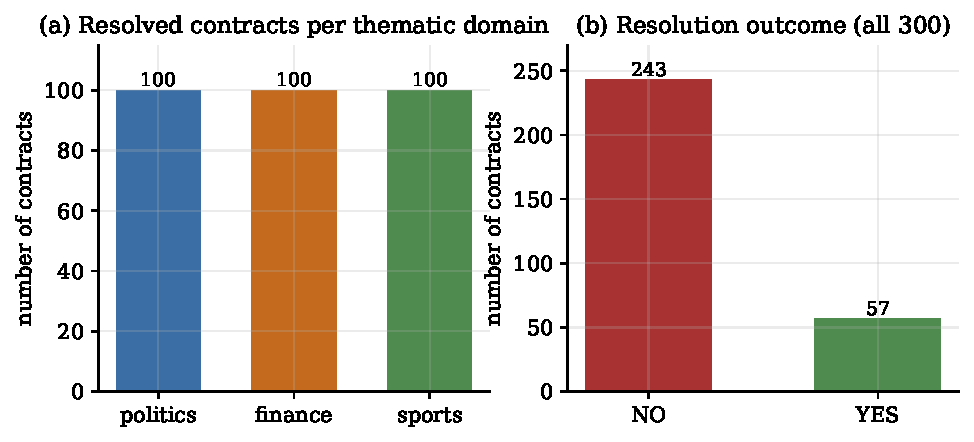
\includegraphics[width=\linewidth]{fig_domain_resolution.pdf}
\caption{The 300-contract study set. (a)~Exactly 100 resolved contracts per thematic
domain. (b)~The resolution outcome is heavily skewed towards \textsc{No}
(243 vs.\ 57), an imbalance that any predictive model must respect.}
\label{fig:domain-res}
\end{figure}

\section{Dataset at a glance}
\Cref{tab:glance} consolidates the headline figures of the constructed dataset; each
is derived in the chapters that follow. Together they make the scale concrete: two
heterogeneous sources, more than 2.7~million primary records before enrichment, and a
fully linked and labelled analytical layer on top.

\begin{table}[H]
\centering
\caption[The constructed dataset at a glance]{The constructed dataset at a glance.
Every figure is regenerated from the persisted pipeline artifacts
(\code{scripts/\_paper\_figs.py}).}
\label{tab:glance}
\small
\begin{tabular}{@{}l r l@{}}
\toprule
\textbf{Artifact} & \textbf{Count} & \textbf{Notes}\\
\midrule
Resolved binary contracts        & 300        & 100 / 100 / 100 by domain\\
Price points                     & 1{,}353{,}114 & full lifetime, 300/300 contracts\\
Social posts (deduplicated)      & 1{,}368{,}041 & Telegram 1{,}348{,}965 + Reddit 16{,}254 + X 2{,}822\\
Distinct channels / subreddits   & 68         & ---\\
Enriched posts                   & 1{,}368{,}041  & sentiment + NER + hashtags + language (all posts)\\
Scored contract--post pairs      & 4{,}112{,}547  & deterministic relevance\\
Accepted evidence links          & 37{,}562   & over 147 contracts\\
Outcome-aware stance labels      & 35{,}679   & over 140 contracts\\
LDA topics                       & 10         & over linked discourse\\
Knowledge-graph relationships    & $>2.7$M    & Neo4j projection\\
\bottomrule
\end{tabular}
\end{table}
